\section{辐射场重构方法比较}
本研究分别采用多层B样条插值重构方法、克里金插值重构方法以及本论文提出的插值重构方法对上一节中模拟的四种辐射场进行插值重构。通过对比重构相对偏差以及重构时间来比较三种插值重构方法的在不同辐射场下的重构效果。

\subsection{辐射场重构相对偏差比较}
多层B样条插值重构算法原理见第二章,是插值算法中常用的一种算法;克里金插值重构算法原理见第三章,是一种多用于地质勘探领域的插值算法;本论文提出的辐射场插值重构算法见第四章,是一种结合多层B样条插值算法和克里金插值算法的创新插值重构算法。下面分别对该三种插值重构算法在单点源无屏蔽空间辐射场、多点源无屏蔽空间辐射场、单点源有屏蔽空间辐射场、多点源有屏蔽空间辐射场进行应用,比较其在不同辐射场中的相对偏差大小。

\begin{figure}[htbp]
    \centering
    \subfigure[多层B样条插值重构]{\includegraphics[width=0.32\textwidth]{figures/Deviation/Spine/SingleSourceUnshielded.jpg}\label{fig:exph7}}
    \subfigure[克里金插值重构]{\includegraphics[width=0.32\textwidth]{figures/Deviation/Kriging/SingleSourceUnshielded.jpg}\label{fig:exgr7}}
    \subfigure[创新插值重构]{\includegraphics[width=0.32\textwidth]{figures/Deviation/RFRMethod/SingleSourceUnshielded.jpg}\label{fig:exls7}}
    \caption{单点源无屏蔽空间辐射场插值重构相对偏差对比}
    \label{单点源无屏蔽空间辐射场插值重构相对偏差对比}
\end{figure}

从图\ref{单点源无屏蔽空间辐射场插值重构相对偏差对比}中可以看出,三种插值算法都能较好的重构出辐射场剂量分布,本论文提出的插值重构方法相比于多层B样条插值重构方法和克里金插值重构方法要略好。

\begin{figure}[htbp]
    \centering
    \subfigure[多层B样条插值重构]{\includegraphics[width=0.32\textwidth]{figures/Deviation/Spine/MultiSourcesUnshielded.jpg}\label{fig:exph8}}
    \subfigure[克里金插值重构]{\includegraphics[width=0.32\textwidth]{figures/Deviation/Kriging/MultiSourcesUnshielded.jpg}\label{fig:exgr8}}
    \subfigure[创新插值重构]{\includegraphics[width=0.32\textwidth]{figures/Deviation/RFRMethod/MultiSourcesUnshielded.jpg}\label{fig:exls8}}
    \caption{多点源无屏蔽空间辐射场插值重构相对偏差对比}
    \label{多点源无屏蔽空间辐射场插值重构相对偏差对比}
\end{figure}

从图\ref{多点源无屏蔽空间辐射场插值重构相对偏差对比}中可以看出,三种插值算法都能不错的重构出辐射场剂量分布,克里金插值重构方法的相对偏差总体要好于多层B样条插值重构方法和本论文提出的插值重构方法,因为在多点源无屏蔽辐射场中,辐射场剂量分布情况通过克里金插值重构方法相比多层B样条插值重构方法更加合适,因此重构结果偏差相对较小。

\begin{figure}[htbp]
    \centering
    \subfigure[多层B样条插值重构]{\includegraphics[width=0.32\textwidth]{figures/Deviation/Spine/SingleSourceshielded.jpg}\label{fig:exph9}}
    \subfigure[克里金插值重构]{\includegraphics[width=0.32\textwidth]{figures/Deviation/Kriging/SingleSourceshielded.jpg}\label{fig:exgr9}}
    \subfigure[创新插值重构]{\includegraphics[width=0.32\textwidth]{figures/Deviation/RFRMethod/SingleSourceshielded.jpg}\label{fig:exls9}}
    \caption{单点源有屏蔽空间辐射场插值重构相对偏差对比}
    \label{单点源有屏蔽空间辐射场插值重构相对偏差对比}
\end{figure}

从图\ref{单点源有屏蔽空间辐射场插值重构相对偏差对比}中可以看出,多层B样条插值重构与模拟结构的相对偏差大于克里金插值重构和本论文提出的辐射场插值重构方法相对偏差,说明在带有屏蔽的辐射场下,样条插值重构方法差于克里金插值重构方法。

\begin{figure}[htbp]
    \centering
    \subfigure[多层B样条插值重构]{\includegraphics[width=0.32\textwidth]{figures/Deviation/Spine/MultiSourcesshielded.jpg}\label{fig:exph10}}
    \subfigure[克里金插值重构]{\includegraphics[width=0.32\textwidth]{figures/Deviation/Kriging/MultiSourcesshielded.jpg}\label{fig:exgr10}}
    \subfigure[创新插值重构]{\includegraphics[width=0.32\textwidth]{figures/Deviation/RFRMethod/MultiSourcesshielded.jpg}\label{fig:exls10}}
    \caption{多点源有屏蔽空间辐射场插值重构相对偏差对比}
    \label{多点源有屏蔽空间辐射场插值重构相对偏差对比}
\end{figure}

从图\ref{多点源有屏蔽空间辐射场插值重构相对偏差对比}中可以看出,三种插值算法都能较好的重构出辐射场剂量分布,本论文提出的插值重构算法重构效果与克里金插值重构算法重构效果相似,略好于样条插值重构算法重构的辐射场结果。

通过对比本论文提出的插值重构方法与多层B样条插值重构方法和克里金插值重构方法的重构相对偏差,发现本论文提出的插值重构方法在某些插值点要明显好于其他两种方法,但在某些插值点也明显。例如在多点源无屏蔽空间辐射场中,存在多层B样条插值重构相对偏差较小的插值点,也存在克里金插值重构相对偏差较小的插值点,亦存在本论文提出的辐射场插值重构相对偏差较小的插值点,如表\ref{不同重构插值方法下辐射场剂量率插值相对偏差比较}所示。通过比较这些插值方法,发现在辐射场剂量分布较为平缓的区域内,多层B样条插值重构出的辐射场与模拟值相对偏差较小;在辐射场剂量分布变化较大的区域,克里金插值重构出的辐射场与模拟值相对偏差较小。

\begin{table}[htbp]
    \centering
    \caption{\label{tab:test3}不同重构插值方法下辐射场剂量率插值相对偏差比较}
    \begin{tabular}{lccc}
        \toprule
        插值坐标(m)             & 多层B样条插值重构(\%) & 克里金插值重构(\%) & 创新插值重构(\%) \\
        \midrule
        $ (-1.45,-0.75,-0.65) $ & 6.81                  & 10.00              & 8.41             \\
        $ (-1.25,1.05,1.95) $   & 1.02                  & 0.86               & 0.01             \\
        $ (0.75,0.05,-0.25) $   & 3.98                  & 0.41               & 2.19             \\
        \bottomrule
    \end{tabular}
    \label{不同重构插值方法下辐射场剂量率插值相对偏差比较}
\end{table}

\subsection{辐射场重构时间比较}
为探究三种辐射场重构方法在重构时间上的关系,将多层B样条插值重构方法、克里金插值重构方法和本论文提出的辐射场插值重构方法分别在以上四种辐射场进行插值,记录其重构所需的时间,结果如表\ref{不同重构插值方法下辐射场重构时间比较}所示。

\begin{table}[htbp]
    \centering
    \caption{\label{tab:test4}不同重构插值方法下辐射场重构时间比较}
    \begin{tabular}{lccc}
        \toprule
        空间辐射场类型   & 多层B样条重构时间(s) & 克里金重构时间(s) & 本论文重构时间(s) \\
        \midrule
        单点源无屏蔽空间 & 1.20776              & 0.000233          & 0.001025          \\
        多点源无屏蔽空间 & 2.02339              & 0.000188          & 0.001567          \\
        单点源有屏蔽空间 & 1.9229               & 0.000169          & 0.00236           \\
        多点源有屏蔽空间 & 1.93904              & 0.000223          & 0.001668          \\
        \bottomrule
    \end{tabular}
    \label{不同重构插值方法下辐射场重构时间比较}
\end{table}

从表\ref{不同重构插值方法下辐射场重构时间比较}中可以看出,三种插值重构方法中克里金插值重构所花费的时间最短,本论文提出的插值重构方法时间其次,多层B样条插值重构时间最长。在实际辐射场重构应用中,该三种方法重构所花费的时间均可。